\apendice{Documentación técnica de programación}

\section{Introducción}

	La idea de este apartado es marcar los pasos a seguir para que cualquier persona que decidiese escalar este trabajo pudiera ejecutarlo sin problema en su equipo. Es importante aclarar que Flutter establece una serie de requirimientos específicos que son de vital importancia para que todo funcione correctamente.

\section{Estructura de directorios}

	La estructura de directorios puede verse representada en la Figura \ref{fig:directorios}. Aunque muchas de las carpetas se crean automáticamente a la hora de crear el proyecto, destacan distintos archivos y directorios creados para la realización del trabajo. Hay que añadir que si no se comentan de manera específica significa que no son archivos donde se hayan realizado cambios y, por consiguiente, no son necesarios tocar si se quisiera escalar la aplicación.
	
\begin{figure}[H]
    \centering
    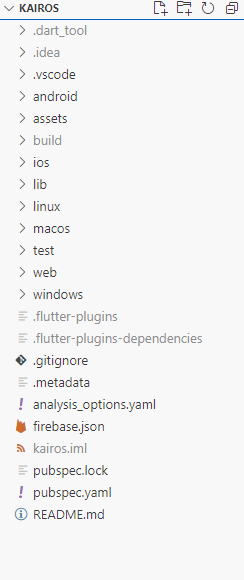
\includegraphics[width=0.5\linewidth]{img/directorios.png}
    \caption{Diseño de aplicar a una subasta y predicción de precio}
    \label{fig:directorios}
\end{figure}

	En la carpeta \emph{assets} se encuentran arhivos de diversos tipos que son necesarios para la realización de la aplicación. En mi caso, la carpeta contiene los siguientes archivos:
	\begin{enumerate}
		\item \textbf{databasewatches.csv :} archivo de extensión csv utilizado para el entrenamiento del modelo de predicción de precios y para cargar los desplegables de campos como \emph{brand}, \emph{model} y \emph{condition} entre otros. Más adelante veremos como se ha conseguido tal tarea.
		\item \textbf{kairoswallpaper.png :} imagen utilizada para establecer el fondo decorativo de la aplicación.
	\end{enumerate}
	
	En la carpeta \emph{lib} encontramos los scripts que han dado vida a la aplicación. Dentro de ella se han creado subdirectorios para seguir un orden y estructura claro. En este caso, los directorios han sido:
	\begin{enumerate}
		\item \textbf{models:} recoge los modelos de la aplicación.
		\item \textbf{views:} recoge los scripts con las vistas y controladores de la aplicación.
		\item \textbf{settings:} recoge scripts con funciones necesarias para traer datos de archivos presentes en la carpeta \emph{assets}.
	\end{enumerate}
	
	Por último, uno de los archivos más importantes es \emph{pubspec.yaml}, donde se definen todas las dependencias con sus versiones necesarias para compilar el programa.

\section{Manual del programador}

	Una vez explicado todo lo que uno debe saber antes de adrentarse en el proyecto, se procede a explicar cómo se ha programado la aplicación.
	
	En la carpeta \emph{models} se encuentran los tres scripts con extensión ``.dart'' que hacen el papel de modelos. Ya se pudo ver en la Figura \ref{fig:db5} y la Figura \ref{fig:db6} que era necesario entablar la comunicación con la base de datos y cómo debía hacerse.
	
	Con esto visto, solo queda explicar las clases ``AuctionRepository'', ``UserRepository'' y ``WatchRepository''. Todas estas clases manejan las operaciones de creación, lectura, actualización y eliminación de objetos según se necesitó para afrontar los requisitos establecidos. Sin embargo, una cosa fundamental que comparten las tres es la instancia de Firebase Firestore dentro de la clase para poder llevar todas estas a cabo, tal y como se representa en la Figura \ref{fig:instanciaFirebase}.

\imagen{instanciaFirebase}{Definición de atributo Firestore}

	Ya que todas las funciones están comentadas y explicar todo haría de este informe una novela, me quiero quedar con cómo se han realizado funciones de consulta de datos a la base de datos. En el caso del modelo ``user.dart'', se necesitó una función que devolviese el dinero de un usuario pasando como parámetro el correo electrónico de este, tal y como se representa en la Figura \ref{fig:consultaMonedero}.
	
\imagen{consultaMonedero}{Forma de consulta de datos a base de datos}

	La forma de consultar datos a base de datos nos obliga, en este caso, a definir una función asíncrona que devolverá eventualmente un entero. En cuanto a la parte de la consulta, se debe especificar la colección a la que se quiere acceder (recordemos que lo que siempre hemos conocido como tablas, aquí son colecciones), la condición que debe cumplir, y limitamos a uno el resultado porque solo debemos recibir un único valor (en este caso la cantidad del dinero asociado a ese correo electrónico). El ``.get()'' será el encargado de devolvernos un ``QuerySnapshot'' con los resultados de la consulta. 
	
	La siguiente comprobación simplemente nos asegura que, si ``QuerySnapshot'' no llegó vacío, devuelva el valor \emph{wallet} del primer documento. Si algo hubiera salido mal, se lanzaría una excepción especificando que el usuario no fue encontrado.
	
	Con las cosas claras de la parte de los modelos, pasamos a la parte de \emph{settings}. Como se ha explicado antes, esta carpeta se destinó a albergar funciones que pudieran ser comunes a varios \emph{scripts} y/o comunicaciones con otros archivos. En este caso, se destinó a albergar el \emph{script} donde se encuentra la función que permite cargar y procesar los datos del archivo con extensión ``.csv'' alojado en la carpeta \emph{assets}.
	
	Tal y como se representa en la Figura \ref{fig:cargaCSV}, la función va a cargar el archivo utilizando una función propia de Flutter y va devolver una lista de mapas con los datos procesados. Es importante tener en cuenta que la primera fila del archivo son los encabezados, por lo que se indica con ``csvTable.skip(1)''. 
	
\imagen{cargaCSV}{Función para extraer datos de dataset}

	En cuanto a las vistas, las funciones quedan explicadas en el código con distintos comentarios donde sean necesarios. Sin embargo, existen ciertas funciones que conviene dejar explciadas en este informe por si surgiese cualquier duda.
	
	Como podemos apreciar en la Figura \ref{fig:responsive}, todos los textos, botones e imágenes de la aplicación van a compartir semejanzas con ella. Es cierto que podría haberse utilizado funciones \emph{responsive} propias de la herramienta, pero durante la realización vimos que afeaba la interfaz ya que los botones tendían a ocupar el largo de la pantalla y, en monitor, no quedaba bonito. Por esta razón, se ideó ajustar el tamaño de los distintos objetos antendiendo al largo de la pantalla.
	
\imagen{responsive}{Forma de hacer la aplicación responsive}

	Otro aspecto importante es la actualización de \emph{widgets} cada vez que viajabamos de una vista a otra y/o realizabamos acciones que necesitaran de un \emph{reload} de la ventana para visualizar los nuevos datos. Un caso lo tenemos en la vista ``home.dart'', donde queremos que el \emph{widget} que presenta el dinero del usuario, se actualice cada vez que viajamos a la venta home. Esto es lo que se representa en la Figura \ref{fig:estadoWallet}. 

\imagen{estadoWallet}{Forma de actualizar un widget}

	Muchas de las cosas predefinidas por Flutter no son intuitivas para el usuario, por lo que se pensó definir una función que controlase la forma de visualizar los mensajes informativos que se den a lo largo de la apliación. Para ello se utiliza la función presentada en la Figura \ref{fig:formaDialogos}, la cual consta de dos partes donde definimos el título del error y una descripción detallada de ello.
	
\imagen{formaDialogos}{Funcion para visualización de diálogos}

	Como hemos indicado en otros apartados, la aplicación cuenta con una llamada a una API, consulta que es necesario definir en el \emph{script} ``addwatch.dart''. Para ello, es importante previamente importar el paquete ``http'', el cual va a permitir que podamos lanzar la consulta, indicando la dirección de la API en la web (alojada en Render). Si el estado de la consulta es 200, todo habrá ido bien. En cambio, si no lo fuese, debemos tratar las excepciones tal y como se plantea en el código. Código en la Figura \ref{fig:llamadaAPI}.

\imagen{llamadaAPI}{Forma de hacer consulta a la API}

	En cuanto a las contraseñas, me pareció una buena idea incluir una función muy presente en muchas webs y aplciaciones: ocultar y mostrar la \emph{password}. Para ello, simplemente definí dos variables booleanas que marcaran si la contraseña se debía mostrar o no en función del pulso sobre el botón definido. Tal código se ve representado en la Figura \ref{fig:ocultarPassword} y la Figura \ref{fig:ocultarPassword2} respectivamente.

\imagen{ocultarPassword}{Variables booleanas para contraseña}
\imagen{ocultarPassword2}{Lógica de ocultar y mostrar contraseña}

	Otro concepto que puede no ser entendido es lo definido como ``regex''. Simplemente se conocen como expresiones regulares y su objetivo es marcar patrones para la manipulación de texto. Mediante su uso, se ha conseguido marcar las validaciones de campos como contraseña, número de cuenta o nombre del usuario, entre otros. Su programación de puede ver en la Figura \ref{fig:validaciones}.
	 
\imagen{validaciones}{Expresiones regulares}

	Por último, no me quería dejar una función importante a la hora de establecer los primeros pasos con Firestore Database. En el script ``main.dart'', en la mayoría de casos, solo se recogen las rutas definidas en la aplicación. Sin embargo, al trabajar con esta base de datos, es necesario definir la función representada en la Figura \ref{fig:inicializacionBaseDeDatos} para que todo funcione correctamente.
	
\imagen{inicializacionBaseDeDatos}{Función que inicializa Firebase}


\section{Compilación, instalación y ejecución del proyecto}

	Para poder ejecutar el proyecto en nuestro equipo, es importante cumplir una serie de requisitos previos e instalar algún que otro programa. Para hacerlo de la manera más estructurada posible, se detallan a continuación los que seguí según \cite{instalacion:flutter}:
	
	\begin{enumerate}
		\item Entramos en sitio web oficial de Flutter \cite{flutter}.
		\item Pulsamos sobre el botón ``Get started''.
		\item Pulsamos sobre el icono de nuestro sistema operativo (en mi caso Windows)
		\item Pulsamos sobre el botón ``Mobile''
		\item Instalamos Visual Studio Code como 
	\end{enumerate}
	
	(Falta completarlo)

%	Antes de explicar como poner el proyecto en nuestro ordenador, me gustaría marcar cuáles han sido los pasos seguidos para crear el proyecto. Esto puede ser de ayuda a futuros estudiantes por su alguno de los pasos a seguir desembocan en errores no comprensibles:
%	\begin{enumerate}
%		\item Desde la consola, nos situamos en la carpeta donde queramos crear el proyecto.
%		\item Escribimos flutter create nombredelproyecto
%		\item Nos situamos en el proyecto.
%		\item Escribimos cmd . para abrir VSC
%	\end{enumerate}
%	
%	Estos serían los pasos principales para la creación del proyecto. Una vez realizados, para conectar Flutter a Firebase, es decir, nuestra base de datos realizamos:
%	\begin{enumerate}
%		\item Vamos a Firebase en nuestro navegador
%		\item Iniciamos sesión
%		\item Pulsamos en el apartado Ir a la consola
%		\item Creamos el proyecto con el nombre que se desee
%		\item Habilitamos análisis y seleccionamos España
%		\item Dentro del apartado compilación creamos firestore database
%		\item Pulsamos sobre crear base de datos
%		\item Marcamos como ubicación eur3(Europe)
%		\item Marcamos comenzar en modo de prueba. Recomendable cambiar el campo fecha manualmente para no perder la base de datos.
%	\end{enumerate}
%	
%	De esta forma, ya habríamos creado la base de datos en la nube. Sin embargo, es necesario comunicar esta con nuestra aplicación Flutter. Para ello:
%	\begin{enumerate}
%		\item En consola, nos situamos en la carpeta del proyecto y escribimos flutter pub add $firebase_core$
%		\item Descargamos aplicación node.
%		\item Ejecutamos como administrador el comando npm install -g $firebase-tools$
%		\item Escribimos firebase login e iniciamos sesión
%		\item Escribimos dart pub global activate $flutterfire-cli$
%		\item Escribimos flutterfire configure
%		\item Con las flechas nos situamos en el proyecto, dejamos marcados todos los campos y marcamos yes
%	\end{enumerate}	

\section{Pruebas del sistema}

(Falta completarlo)